\section{Aufbau}
\label{sec:Aufbau}
\begin{figure}
	\centering
	\caption{Skizze des Versuchsaufbaus \cite{V406}.}
	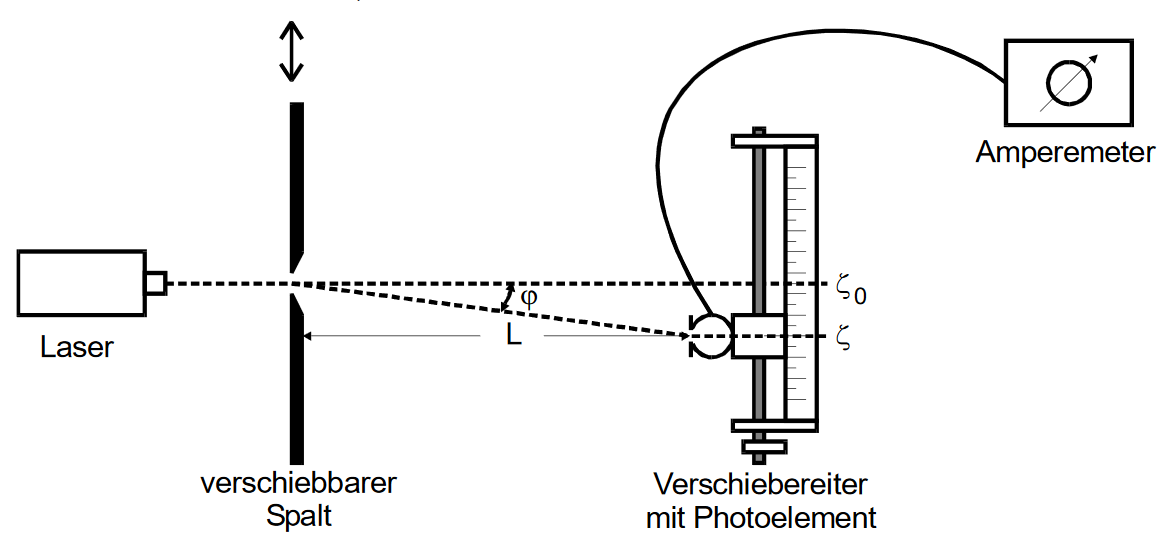
\includegraphics[width=\linewidth-150pt,height=\textheight-150pt,keepaspectratio]{content/images/Aufbau.png}
	\label{fig:Aufbau}
\end{figure}
In den theoretischen Überlegungen sind wir von kohärentem und monochromatischem Licht ausgegangen. Dies wird im Versuchsaufbau in guter Näherung durch einen He-Ne-Laser mit einer Wellenlänge $\lambda = \SI{633}{\nano\meter}$ realisiert. Dieser trifft senkrecht auf einen Einzel- bzw. Doppelspalt, an welchem das Licht gebeugt wird. In einer Entfernung von ca. $\SI{130}{\centi\meter}$ zur Blende befindet sich ein Verschiebereiter mit Photoelement. Das Photoelement gibt einen Strom ab der proportional zur auftreffenden Lichtintensität ist. Diese Strom kann an einem Nanoamperemeter abgelesen werden.